\documentclass[12pt]{report}

\usepackage[utf8]{inputenc}
\usepackage{graphicx}
\usepackage{geometry}
\usepackage{vmargin}
\usepackage{float}
\usepackage{wrapfig}
\usepackage[dvipsnames]{xcolor}
\usepackage{listings}
\usepackage{fancyhdr}
\usepackage[acronym,nomain,nonumberlist]{glossaries}
\usepackage{setspace}
\usepackage{hyperref}
\usepackage{array}
\usepackage{multicol}
\usepackage[belowskip=-10pt]{caption}
\usepackage{subcaption}
\usepackage{enumitem}
\usepackage[spanish]{babel}
\usepackage[backend=biber,style=iso-numeric]{biblatex}
\addbibresource{refs.bib}


% Document margins
\setpapersize{A4}
\setmargins{2.2cm}          % margen izquierdo
{0cm}                       % margen superior
{16.5cm}                    % anchura del texto
{24.57cm}                   % altura del texto
{55pt}                      % altura cabeceras
{1.25cm}                    % espacio entre el texto y los cabeceras
{1pt}                       % altura del pie de página
{1cm}                       % Espacio entre el texto y el pie de página

% Line spacing
\renewcommand{\baselinestretch}{1.5} 

% Remove paragraph indentation
\setlength{\parindent}{0pt}

% Paragraph spacing
\setlength{\parskip}{1em}

% Definir colores personalizados
\definecolor{linkcolor}{RGB}{52, 152, 219}   % Azul claro
\definecolor{citecolor}{RGB}{231, 76, 60}    % Rojo suave
\definecolor{urlcolor}{RGB}{46, 204, 113}    % Verde esmeralda
\definecolor{filecolor}{RGB}{155, 89, 182}   % Morado
\definecolor{menucolor}{RGB}{241, 196, 15}   % Amarillo dorado
\definecolor{codegray}{gray}{0.95}           % Gris claro para el código

% Configuración de Hyperref con colores
\hypersetup{
    colorlinks=true,
    linkcolor=linkcolor,
    citecolor=citecolor,
    urlcolor=linkcolor,
    filecolor=filecolor,
    menucolor=menucolor,
    bookmarksopen=true,
    bookmarksnumbered=true,
    pdfstartview=FitH,
    pdfpagemode=UseOutlines
}

% Configuración de los fragmentos de código
\lstdefinestyle{mystyle}{
    backgroundcolor=\color{white},       % Fondo blanco
    basicstyle=\ttfamily\footnotesize,   % Fuente monoespaciada y pequeña
    keywordstyle=\color{RoyalBlue},      % Palabras clave en azul
    commentstyle=\color{ForestGreen},    % Comentarios en verde oscuro
    stringstyle=\color{BrickRed},        % Strings en rojo ladrillo
    numberstyle=\tiny\color{gray},       % Números de línea en gris
    frame=tb,                            % Marco arriba y abajo
    rulecolor=\color{gray},              % Color del marco
    aboveskip=3mm,
    belowskip=3mm,
    tabsize=4,
    showstringspaces=false,
    showspaces=false,
    showtabs=false,
    breaklines=true,
    breakatwhitespace=false,
    escapeinside={\%*}{*)},
    keepspaces=true,
    captionpos=b,
    framexleftmargin=16pt,
    framextopmargin=3pt,
    framexbottommargin=6pt,
    extendedchars=true,
    title=\lstname
}

\lstset{style=mystyle}

\colorlet{punct}{red!60!black}
\definecolor{background}{HTML}{EEEEEE}
\definecolor{delim}{RGB}{20,105,176}
\colorlet{numb}{magenta!60!black}

\lstdefinelanguage{json}{
    stepnumber=1,
    numbersep=8pt,
    showstringspaces=false,
    breaklines=true,
    frame=lines,
    backgroundcolor=\color{white},
    aboveskip=0mm,
    belowskip=0mm,
    literate=
     *{0}{{{\color{numb}0}}}{1}
      {1}{{{\color{numb}1}}}{1}
      {2}{{{\color{numb}2}}}{1}
      {3}{{{\color{numb}3}}}{1}
      {4}{{{\color{numb}4}}}{1}
      {5}{{{\color{numb}5}}}{1}
      {6}{{{\color{numb}6}}}{1}
      {7}{{{\color{numb}7}}}{1}
      {8}{{{\color{numb}8}}}{1}
      {9}{{{\color{numb}9}}}{1}
      {:}{{{\color{punct}{:}}}}{1}
      {,}{{{\color{punct}{,}}}}{1}
      {\{}{{{\color{delim}{\{}}}}{1}
      {\}}{{{\color{delim}{\}}}}}{1}
      {[}{{{\color{delim}{[}}}}{1}
      {]}{{{\color{delim}{]}}}}{1},
}

% Reducir el espacio entre líneas en listas
\setlist[itemize]{nosep, topsep=0pt, partopsep=0pt}

% Header  configuration
\pagestyle{fancy}
\fancypagestyle{plain}{
    \fancyhf{}
    \rhead{{Desarrollo de una aplicación web para la gestión \\ centralizada de múltiples marketplaces}}
    \lhead{
\includegraphics[width=5cm]{figures/generic/logo_eseiaat.png}}
    \cfoot{\thepage}
}
\fancyhf{}
\rhead{{Desarrollo de una aplicación web para la gestión \\ centralizada de múltiples marketplaces}}
\lhead{
\includegraphics[width=5cm]{figures/generic/logo_eseiaat.png}}
\cfoot{\thepage}

% Create acronym list
\makenoidxglossaries
\newacronym{sku}{SKU}{Stock Keeping Unit}
\newacronym{api}{API}{Application Programming Interface}
\newacronym{crm}{CRM}{Customer Relationship Management}
\newacronym{orm}{ORM}{Object Relational Mapping}
\newacronym{sql}{SQL}{Structured Query Language}
\newacronym{html}{HTML}{HyperText Markup Language}
\newacronym{css}{CSS}{Cascading Style Sheets}
\newacronym{mvc}{MVC}{Modelo-Vista-Controlador}
\newacronym{json}{JSON}{JavaScript Object Notation}
\newacronym{rest}{REST}{Representational State Transfer}

\begin{document}

% Rename of variables
\renewcommand{\listfigurename}{Índice de figuras}
\renewcommand{\listtablename}{Índice de tablas}
\renewcommand{\contentsname}{Sumario}
\renewcommand{\figurename}{Figura}
\renewcommand{\tablename}{Tabla}
\renewcommand{\chaptername}{Capítulo}
\renewcommand{\bibname}{Referencias}
\renewcommand*{\acronymname}{Acrónimos}
\renewcommand{\lstlistingname}{Fragmento}


\pagenumbering{gobble}
\newgeometry{left=5cm,bottom=0.1cm,textwidth=19cm}

{
    \setstretch{1}
    \parskip=0pt
    \fontsize{10pt}{12pt}

    \pagestyle{empty}

    \begin{figure}[h]
        
\includegraphics[width=6cm]{figures/generic/logo_eseiaat.png}
    \end{figure}

    \begin{wrapfigure}{r}{0.25\textwidth}
        \centering
        
\includegraphics[angle=90, width=0.07\textwidth]{figures/generic/Trabajofindeestudios.jpg}
    \end{wrapfigure}

    \phantom{abs}

    \vspace{1.5cm}

    \textbf{\scalebox{2.5}{\textcolor{RoyalBlue}{\parbox{\textwidth}{Desarrollo de una aplicación web \\ para la gestión centralizada de \\ múltiples marketplaces}}}}

    \vspace{2cm}

    \textbf{\scalebox{1.5}{{Documento:}}}

    \vspace{0.5 cm}
    \scalebox{1.5}{\textcolor{RoyalBlue}{Memoria}}

    \vspace{2cm}

    \textbf{\scalebox{1.5}{{Autor/Autora:}}}

    \vspace{0.5 cm}
    \scalebox{1.5}{{\textcolor{RoyalBlue}{Aleix Ribas Torras}}}

    \vspace{2cm}

    \textbf{\scalebox{1.5}{{Director/Directora - Codirector/Codirectora:}}}

    \vspace{0.5 cm}
    \scalebox{1.5}{\textcolor{RoyalBlue}{\parbox{\textwidth}{Francisco José Múgica Alvarez \\ Maria Angela Nebot Castells}}}

    \vspace{2cm}

    \textbf{\scalebox{1.5}{{Titulación:}}}

    \vspace{0.5 cm}
    \scalebox{1.5}{{\textcolor{RoyalBlue}{Grado en Ingeniería en Tecnologías Aeroespaciales}}}

    \vspace{2cm}

    \textbf{\scalebox{1.5}{{Convocatoria:}}}

    \vspace{0.5 cm}

    \scalebox{1.5}{{\textcolor{RoyalBlue}{Primavera, 2025}}}

}

\restoregeometry

\newpage
\thispagestyle{empty}
\phantom{abc}
\newpage

\pagenumbering{Roman}

\chapter*{Resumen}
El presente proyecto desarrolla una aplicación web para la gestión centralizada de múltiples marketplaces, concebida como una potente herramienta de automatización y un método unificado para optimizar las operaciones de comercio electrónico. El sector del e-commerce, en constante crecimiento, enfrenta desafíos significativos como la feroz competencia, la complejidad de la infraestructura tecnológica y logística, y los altos costos asociados a la administración de productos, pedidos y pagos en diversos canales de venta, lo que tradicionalmente consume valiosos recursos y tiempo.

Para superar estos obstáculos y aprovechar las oportunidades del comercio en línea, la solución propuesta actúa como un método estratégico y centralizado para administrar eficientemente los canales de venta. Su objetivo principal es centralizar la información y la gestión de pedidos y productos de diferentes marketplaces en una única plataforma, ofreciendo una visión unificada del negocio.

Esta solución representa una primera versión funcional que sienta las bases para lo que, en el futuro, podría evolucionar hacia una plataforma integral de gestión multicanal, capaz de escalar, adaptarse a nuevos marketplaces y ofrecer herramientas avanzadas de análisis, automatización y toma de decisiones para los comercios electrónicos.

\chapter*{Abstract}
This project develops a web application for the centralized management of multiple marketplaces, conceived as a powerful automation tool and a unified method to optimize e-commerce operations. The e-commerce sector, which is constantly growing, faces significant challenges such as an strong competition, the complexity of technological and logistical infrastructure, and the high costs associated with managing products, orders, and payments across various sales channels, raditionally consuming valuable time and resources.

To overcome these obstacles and seize the opportunities of online commerce, the proposed solution acts as a strategic and centralized method for efficiently managing sales channels. Its main goal is to centralize information and the management of orders and products from different marketplaces into a single platform, offering a unified view of the business.

This solution represents a first functional version that lays the groundwork for what could, in the future, evolve into a comprehensive multichannel management platform, capable of scaling, adapting to new marketplaces, and providing advanced tools for analysis, automation, and decision-making for e-commerce businesses.

\selectlanguage{spanish}

\tableofcontents
\listoffigures
\glsaddall
\renewcommand{\thepage}{\Roman{page}}
\printnoidxglossaries

\newpage
\pagenumbering{arabic}
\renewcommand{\thepage}{\arabic{page}}

\chapter{Introducción}
\label{chap:intro}
\chapter{Marco Teórico}
\label{chap:marco_teorico}

En este capítulo se presenta el marco teórico que sustenta el desarrollo de la aplicación web para la gestión centralizada de múltiples \textit{marketplaces}. Se abordan conceptos clave relacionados con el comercio en línea, sus dificultades y sus múltiples vertientes. Además, se exploran las tecnologías y herramientas utilizadas en el desarrollo de la aplicación, así como las metodologías de trabajo adoptadas durante el proceso.

\section{Comercio electrónico y canales de venta en línea}
\label{sec:comercio_canales}

En los últimos años, el comercio electrónico se ha convertido en una parte fundamental de la economía global. La capacidad de comprar y vender productos y servicios a través de internet ha transformado la forma en que las empresas interactúan con sus clientes. Este fenómeno ha dado lugar a la aparición de nuevos canales de venta, los llamados canales de venta en línea, que permiten a las empresas llegar a un público más amplio y diversificado, donde antes dependían de tiendas físicas o distribuidores locales.

No obstante, el comercio electrónico no es tan fácil como puede parecer en primera instancia. Existen tres grandes desafíos que las empresas deben enfrentar: la competencia, la infraestructura tecnológica y logística.

En internet todo el mundo juega con las mismas reglas; las facilidades que ofrece este medio son iguales para todos. El factor de proximidad al cliente ya no es el diferencial, sino la capacidad de ofrecer un producto o servicio que se diferencie del resto, tanto en calidad, precio o experiencia de compra. Esto genera que la competencia sea feroz, y las empresas deben encontrar formas innovadoras de destacar entre la multitud, tal como podrían ser las promociones, el marketing digital o la experiencia de usuario.

Por otro lado, el comercio electrónico requiere de una infraestructura tecnológica que permita listar productos, gestionar pedidos y pagos, y mantener una comunicación fluida con los clientes. Esto implica no solo contar con un sitio web atractivo y funcional, sino también con sistemas de gestión de inventario, plataformas de pago seguras y herramientas de análisis de datos que permitan tomar decisiones informadas. Todo esto puede resultar costoso y complicado de implementar, especialmente para pequeñas y medianas empresas que no cuentan con los recursos necesarios, ni en términos de personal, ni de dinero.

Por último, la logística es otro de los grandes retos del comercio electrónico. En el comercio tradicional, los productos se entregan directamente al cliente en la tienda. En el comercio electrónico, las empresas deben gestionar el almacenamiento, el envío y la entrega de productos a los clientes, lo que puede resultar complicado y costoso. La gestión de inventarios, la selección de proveedores de transporte y la coordinación de envíos son solo algunos de los aspectos logísticos que las empresas deben tener en cuenta para garantizar una experiencia de compra satisfactoria que cumpla con las expectativas de los clientes.

Estos tres factores son solo algunos de los muchos desafíos que enfrentan las empresas en el comercio electrónico. Por este mismo motivo, diferentes soluciones han surgido para ayudar a las empresas a superar estos obstáculos y aprovechar al máximo las oportunidades que ofrece el comercio en línea. Entre estas soluciones se encuentran dos que destacan por encima de las demás: las plataformas \textit{e-commerce} y los \textit{marketplaces}. Ambas ofrecen a las empresas la posibilidad de vender sus productos y servicios en línea, pero lo hacen de maneras diferentes.

\subsection{Plataformas \textit{E-commerce}}

Diseñar y programar una tienda en línea desde cero puede ser un proceso largo y costoso. Una tienda en línea no es una simple página web, sino un sistema complejo que debe gestionar una gran cantidad de información, como productos, precios, inventarios, pedidos y clientes.

Muchas empresas optan por utilizar las llamadas plataformas \textit{e-commerce}. Una plataforma \textit{e-commerce} es una aplicación que permite a las empresas crear y gestionar su propia tienda en línea en relativamente pocos pasos. Existen muchas plataformas \textit{e-commerce}, pero todas se caracterizan por ofrecer una serie de herramientas y funcionalidades por defecto de manera que las empresas puedan crear su tienda en línea sin necesidad de tener conocimientos técnicos avanzados. Estas plataformas suelen incluir plantillas de diseño, sistemas de gestión de inventario, herramientas de marketing y análisis, y opciones de pago seguras. Además, muchas de ellas ofrecen integraciones con otros servicios y funcionalidades adicionales, todo bajo los llamados \textit{plugins} \cite{adobe_ecommerce_platforms}.

Todo este conjunto de facilidades hacen que el uso de plataformas \textit{e-commerce} sea una opción atractiva para muchas empresas, especialmente para aquellas que están comenzando en el comercio electrónico o que no cuentan con los recursos necesarios para desarrollar su propia tienda en línea desde cero. Sin embargo, también existen desventajas asociadas al uso de estas plataformas. Por ejemplo, las empresas pueden tener menos control sobre el diseño y la funcionalidad de su tienda en línea, y pueden estar sujetas a las políticas y tarifas de la plataforma, entre muchas otras cosas. Además, algunas plataformas pueden no ser escalables o flexibles lo suficiente como para adaptarse a las necesidades cambiantes de una empresa en crecimiento.

Existe una amplia variedad de plataformas \textit{e-commerce} en el mercado, cada una con sus propias características y funcionalidades. Algunas de las más populares son Shopify, WooCommerce (\textit{plugin} de WordPress), Magento y PrestaShop. Cada una de estas plataformas tiene sus propias ventajas y desventajas, y la elección de la plataforma adecuada dependerá de las necesidades, objetivos específicos y las dimensiones de cada empresa.

\subsection{\textit{Marketplaces}}

Los \textit{marketplaces} son plataformas en línea que permiten a las empresas vender sus productos y servicios a través de un canal de venta compartido. A diferencia de las plataformas \textit{e-commerce}, donde las empresas crean y gestionan su propia tienda en línea, los \textit{marketplaces} permiten a las empresas listar sus productos y servicios junto con los de otras empresas en una única plataforma. Esto significa que las empresas pueden aprovechar la audiencia y el tráfico del \textit{marketplace} para llegar a nuevos clientes sin necesidad de invertir en marketing o publicidad.

Aquí radica realmente la ventaja de los \textit{marketplaces}: la posibilidad de llegar a un público más amplio y diversificado sin necesidad de invertir grandes cantidades de dinero en marketing o publicidad. Tanto en los \textit{e-commerce} tradicionales (tiendas en línea creadas desde cero) como en las plataformas \textit{e-commerce}, las empresas deben invertir considerables cantidades de dinero para atraer tráfico a su tienda en línea, mientras que en los \textit{marketplaces} el tráfico ya está allí, lo que significa que las empresas pueden aprovecharlo para aumentar sus ventas y llegar a nuevos clientes.

No obstante, este tipo de plataformas también tienen sus desventajas. En primer lugar, todos los productos acostumbran a estar bajo una comisión de manera que la empresa o bien debe subir el precio de su producto o asumir la pérdida de margen. Está comisión puede rondar entre el 10\% y el 20\%. En segundo lugar, los \textit{marketplaces} pueden ser muy competitivos, pues un mismo producto puede ser vendido por distintas empresas, dando lugar a una guerra de precios que puede afectar la rentabilidad de las empresas. Por último, en un \textit{marketplace} la empresa no tiene ningún tipo de control sobre la experiencia de compra del cliente, lo que puede afectar la percepción de la marca y la lealtad del cliente, además de que debe someterse a la política de la plataforma, que muchas veces puede no ser beneficiosa para la empresa y puede llegar a afectar sus operaciones.

Existen múltiples \textit{marketplaces}, tanto de productos físicos, como Amazon, eBay o AliExpress, como de productos digitales o servicios, como Udemy, Uber o Glovo. Cada uno de estos tiene sus propias características y funcionalidades, y la elección del \textit{marketplace} adecuado dependerá de las necesidades y objetivos específicos de cada empresa. Es importante destacar que el uso de una plataforma \textit{e-commerce} no excluye la posibilidad de listar productos o servicios en un \textit{marketplace}. De hecho, muchas empresas optan por combinar ambas estrategias para maximizar su alcance y diversificar sus canales de venta, aprovechando las ventajas que ofrece cada una de estas opciones \cite{sharetribe_marketplac_platforms}.
\chapter{Diseño y Desarrollo de la plataforma}
\label{chap:diseno_desarrollo}

En este capítulo se explicará todo el proceso de diseño y desarrollo de la plataforma, dando especial énfasis a la justificación de las decisiones tomadas y a la explicación de los distintos problemas que se han ido encontrando a lo largo del proceso. En concreto, se detallará el diseño de la base de datos, el desarrollo del \textit{backend} y el desarrollo del \textit{frontend}. No obstante, antes de entrar en detalle en cada una de estas secciones, se explicará el proceso inicial de desarrollo de la plataforma y se justificarán las tecnologías elegidas, cumplimentando así la sección \ref{sec:arquitectura_sistema} del capítulo \ref{chap:marco_teorico}.

% \textcolor{red}{Explicar que s'ha decidit fer un saas i una app web degut a les aventatges anteriorment esmentades.}

% \textcolor{red}{Ja s'ha dit que es farà servir React i Django i s'ha explicat breument com funcionen. Afegir el perquè d'aquestes eleccions.}

\section{Proceso inicial de desarrollo de la plataforma}
\label{sec:proceso_desarrollo}

El desarrollo de la aplicación web no surge de simplemente decidir qué tecnologías se van a utilizar y empezar a programar. Antes de comenzar a desarrollar la plataforma se ha llevado a cabo un proceso de diseño que ha permitido definir la arquitectura del sistema, las tecnologías a utilizar y el flujo de trabajo.

\subsection{Separación de tecnologías \textit{frontend} y \textit{backend}}

El primer paso que se ha realizado y una vez ya definido el objetivo de la aplicación y las funcionalidades que se querían implementar, se ha llevado a cabo un análisis de como estructurar la plataforma. Como ya se ha comentado en la sección \ref{sec:arquitectura_sistema}, se ha optado por una arquitectura dividida en dos partes: el \textit{backend}, incluyendo la base de datos, y el \textit{frontend}. No obstante, a pesar de que Django ofrece la posibilidad de crear ambas partes, se ha decidido utilizar React. Esta decisión ha supuesto un reto, ya que ha significado realizar un \textit{frontend} entero además de preparar una API en el \textit{backend} para que ambos se puedan comunicar. Sin embargo, esta decisión ha permitido crear una aplicación más escalable, flexible y, sobre todo, dinámica.

Django es un \textit{framework} que funciona del lado del servidor, lo que significa que cada vez que se quiere mostrar una página distinta, el servidor tiene que procesar la petición y devolver la página completa. De esta manera, cuando el usuario cambia de página, el servidor carga todos los recursos (HTML, CSS y JavaScript) y los rellena con los datos necesarios, sirviendo una página estática. Por el contrario, React es un \textit{framework} que funciona del lado del cliente, lo que significa que el servidor solo tiene que enviar los datos necesarios y el cliente se encarga de mostrar la información. Con esto, el servidor solo tiene que enviar los datos necesarios y el cliente se encarga de mostrar la información. Esto permite crear aplicaciones más dinámicas y rápidas, ya que no es necesario recargar la página cada vez que se quiere mostrar un nuevo contenido.

Este enfoque, a pesar de ser más complejo, es el estándar en la actualidad y es por este motivo que se ha optado por esta división de tecnologías.

\section{Diseño de la base de datos}
\label{sec:diseno_base_datos}

Para estructurar el proyecto, se ha optado por empezar definiendo la base de datos. Diseñar la base de datos inicialmente permite tener una visión general de como se va a estructurar el proyecto y como sus distintas partes se van a relacionar entre sí. Al fin y al cabo, la base de datos es el núcleo de la aplicación, ya que de ella dependen todas las funcionalidades.

En concreto, para el proyecto se ha decidido hacer uso del sistema de gestión de bases de datos PostgreSQL. Esta elección es resultado de la experiencia previa que he tenido con este sistema, ya que he trabajado con él en proyectos anteriores y me he familiarizado con su funcionamiento. Además, PostgreSQL es un sistema de código abierto, lo que significa que es gratuito y se puede utilizar sin restricciones, además de ser muy robusto y escalable, lo que lo hace ideal para aplicaciones de gran tamaño, como podría ser esta en un futuro. Por último, es el sistema más recomendado por Django, lo que facilita la integración entre ambos.

\subsection{Bloques de funcionalidades}

Antes de empezar a diseñar la base de datos, se deben definir los bloques claves de la aplicación para así poder estructurar los datos de manera que se puedan implementar de la mejor manera posible. En este caso, los bloques claves son los siguientes:

\begin{itemize}
    \item \textbf{Bloque de canales:} La herramienta debe permitir la gestión de los distintos canales de venta en línea. Aunque el usuario no crea ni edita de manera directa los canales de venta, interactúa con ellos, de manera que su información debe estar almacenada en la base de datos.
    \item \textbf{Bloque de pedidos:} La herramienta debe centralizar todos los pedidos de los distintos canales de venta en línea y permitir la gestión de los mismos. Esto incluye la posibilidad de crear, editar y eliminar pedidos, así como la posibilidad de marcar un pedido como enviado o entregado.
    \item \textbf{Bloque de productos:} La herramienta debe permitir la gestión de los productos disponibles en los distintos canales de venta en línea. Esto incluye la posibilidad de crear, editar y eliminar productos de los distintos canales, así como la posibilidad de editar sus atributos, tales como el precio, la descripción y la imagen, entre muchos otros.
    \item \textbf{Bloque de usuarios:} La herramienta debe permitir la gestión de los usuarios que pueden acceder a la aplicación. Esto incluye la posibilidad de crear, editar y eliminar usuarios, así como la posibilidad de asignarles distintos permisos y roles dentro de la aplicación.
\end{itemize}

Con los bloques clave definidos, se puede concluir que la base de datos debe contener cuatro tablas principales: una para los pedidos, otra para los productos, otra para los canales y una última para los usuarios. A partir de aquí, se pueden definir las distintas tablas que van a complementar las principales.

Adicionalmente, dado que para este proyecto la aplicación se presenta como una fase inicial de una desarrollo mucho más grande, que en un futuro podría convertirse en una solución comercializable, es indispensable tener en cuenta la escalabilidad de toda la aplicación. Por este motivo, los cuatro bloques que a continuación se detallarán han sido diseñados de manera que se puedan ampliar en un futuro sin necesidad de realizar cambios significativos en la base de datos.

\subsubsection{Bloque de canales de venta}

El bloque de canales de venta es el conjunto de tablas y relaciones que almacenan toda la información correspondiente a los distintos canales de venta en línea. El usuario no interactúa directamente con los canales de venta, es decir, no los crea ni los edita, pero sí que interactúa con ellos al sincronizarlos con sus pedidos y productos.

Este bloque es el más claro ejemplo de la escalabilidad de la aplicación y de la base de datos, ya que trata a cada canal de venta como una entidad independiente, lo que permite añadir nuevos canales sin necesidad de realizar cambios a la estructura de la base de datos.

Este bloque está formado únicamente por una tabla, que es la siguiente:
\begin{itemize}
    \item \textbf{Canal de venta [\texttt{marketplace}]:} Esta tabla almacena la información de los distintos canales de venta en línea. Los campos que contiene son los siguientes:
          \begin{itemize}
              \item \texttt{id}: Identificador único del canal de venta. \textit{Clave primaria (entero)}.
              \item \texttt{name}: Nombre del canal de venta. \textit{Cadena de caracteres}.
              \item \texttt{logo\_url}: URL del logo del canal de venta. \textit{Cadena de caracteres}.
              \item \texttt{color}: Color del canal de venta. \textit{Cadena de caracteres}.
              \item \texttt{country}: País del canal de venta. \textit{Entero}.
          \end{itemize}
\end{itemize}

Con la tabla definida, se puede describir el funcionamiento del bloque. El desarrollador de la aplicación puede añadir nuevos canales de venta añadiendo nuevas filas a la tabla. Este enfoque permite que nuevos canales de venta puedan ser añadidos sin necesidad de hacer grandes cambios en la aplicación, pues cada canal de venta es tratado como una entidad independiente. Al añadir un nuevo canal de venta el usuario verá el nuevo canal en la aplicación tal como si fuera uno ya existente, pudiendo sincronizar sus pedidos y productos con él.

\subsubsection{Bloque de pedidos}

El bloque de pedidos es el conjunto de tablas y relaciones que almacenan toda la información correspondiente a los pedidos. En cada pedido es importante almacenar la información de éste, como el estado, la fecha, el método de pago, el canal de venta, entre otros. Además, para saber donde se debe enviar el pedido, es importante almacenar la información del cliente, como su nombre, dirección y teléfono. Por último, también es importante almacenar la información de los productos que componen el pedido, como su nombre, precio y cantidad solicitada.

Conociendo la información que se debe almacenar, se pueden definir las siguientes tablas:

\begin{itemize}
    \item \textbf{Pedido [\texttt{order}]:} Esta tabla almacena la información general de cada pedido. Los campos que contiene son los siguientes:
          \begin{itemize}
              \item \texttt{id}: Identificador único del pedido. \textit{Clave primaria (entero)}.
              \item \texttt{order\_id}: Identificador del pedido en el canal de venta. \textit{Cadena de caracteres}.
              \item \texttt{status}: Estado del pedido (pendiente, enviado, entregado, cancelado). \textit{Entero}.
              \item \texttt{order\_date}: Fecha en la que se realizó el pedido. \textit{Fecha y hora}.
              \item \texttt{total\_price}: Precio total del pedido. \textit{Decimal}.
              \item \texttt{ticket}: Número de ticket del pedido. \textit{Cadena de caracteres}.
              \item \texttt{ticket\_refund}: Número de ticket de la devolución del pedido. \textit{Cadena de caracteres}.
              \item \texttt{pay\_method}: Método de pago del pedido (tarjeta, transferencia, efectivo). \textit{Entero}.
              \item \texttt{package\_quantity}: Cantidad de bultos (paquetes) del pedido. \textit{Entero}.
              \item \texttt{weight}: Peso del pedido. \textit{Decimal}.
              \item \texttt{notes}: Notas del pedido. \textit{Cadena de caracteres}.
              \item \texttt{origin}: Origen del pedido (creado automáticamente, importado, manual). \textit{Entero}.
              \item \texttt{updated\_at}: Fecha de la última actualización del pedido. \textit{Fecha y hora}.
              \item \texttt{carrier\_id}: Identificador del transportista del pedido. \textit{Entero y relación N:1 con la tabla} \texttt{carrier}.
              \item \texttt{customer\_id}: Identificador del cliente del pedido. \textit{Entero y relación N:1 con la tabla} \texttt{customer}.
              \item \texttt{marketplace\_id}: Identificador del canal de venta del pedido. \textit{Entero y relación N:1 con la tabla} \texttt{marketplace}.
          \end{itemize}
    \item \textbf{Cliente [\texttt{customer}]:} Esta tabla almacena la información del cliente. Se divide entre información de facturación e información de envío, ya que es habitual que los canales de venta permitan añadir ambos tipos de información. Los campos que contiene son los siguientes:
          \begin{itemize}
              \item \texttt{id}: Identificador único del cliente. \textit{Clave primaria (entero)}.
              \item \texttt{bill\_phone}: Teléfono de facturación. \textit{Cadena de caracteres}.
              \item \texttt{bill\_email}: Correo electrónico de facturación. \textit{Cadena de caracteres}.
              \item \texttt{bill\_firstname}: Nombre del cliente para la facturación. \textit{Cadena de caracteres}.
              \item \texttt{bill\_lastname}: Apellido del cliente para la facturación. \textit{Cadena de caracteres}.
              \item \texttt{bill\_company}: Empresa del cliente para la facturación. \textit{Cadena de caracteres}.
              \item \texttt{bill\_address}: Dirección de facturación. \textit{Cadena de caracteres}.
              \item \texttt{bill\_city}: Ciudad de facturación. \textit{Cadena de caracteres}.
              \item \texttt{bill\_zipcode}: Código postal de facturación. \textit{Cadena de caracteres}.
              \item \texttt{bill\_country}: País de facturación. \textit{Entero}.
              \item \texttt{ship\_phone}: Teléfono de envío. \textit{Cadena de caracteres}.
              \item \texttt{ship\_email}: Correo electrónico de envío. \textit{Cadena de caracteres}.
              \item \texttt{ship\_firstname}: Nombre del cliente para el envío. \textit{Cadena de caracteres}.
              \item \texttt{ship\_lastname}: Apellido del cliente para el envío. \textit{Cadena de caracteres}.
              \item \texttt{ship\_company}: Empresa del cliente para el envío. \textit{Cadena de caracteres}.
              \item \texttt{ship\_address}: Dirección de envío. \textit{Cadena de caracteres}.
              \item \texttt{ship\_city}: Ciudad de envío. \textit{Cadena de caracteres}.
              \item \texttt{ship\_zipcode}: Código postal de envío. \textit{Cadena de caracteres}.
              \item \texttt{ship\_country}: País de envío. \textit{Entero pequeño}.
          \end{itemize}
    \item \textbf{Artículo [\texttt{orderitem}]:} Esta tabla almacena la información de los productos que componen el pedido. Los campos que contiene son los siguientes:
          \begin{itemize}
              \item \texttt{id}: Identificador único del artículo. \textit{Clave primaria (entero)}.
              \item \texttt{order\_id}: Identificador del pedido al que pertenece el artículo. \textit{Entero y relación N:1 con la tabla} \texttt{order}.
              \item \texttt{marketplace\_product\_id}: Identificador del producto del artículo. \textit{Entero y relación N:1 con la tabla} \texttt{marketplace\_product}.
              \item \texttt{purchase\_price}: Precio del producto en el momento que se adquirió. \textit{Decimal}.
              \item \texttt{quantity}: Cantidad solicitada del producto del artículo. \textit{Entero}.
          \end{itemize}
    \item \textbf{Transportista [\texttt{carrier}]:} Esta tabla almacena la información de los transportistas. Los campos que contiene son los siguientes:
          \begin{itemize}
              \item \texttt{id}: Identificador único del transportista. \textit{Clave primaria (entero)}.
              \item \texttt{name}: Nombre del transportista. \textit{Cadena de caracteres}.
          \end{itemize}
\end{itemize}

Con esto, se puede observar que el bloque está formado por una tabla principal, la de pedidos \texttt{order}, que almacena la información general de cada pedido, y tres tablas complementarias: la de clientes \texttt{customer}, que almacena la información del cliente, la de artículos \texttt{orderitem}, que almacena la información de los productos que componen el pedido, y la de transportistas \texttt{carrier}, que almacena la información de los transportistas.

Si bien es cierto que la tabla de cliente podría parecer ser redundante, pues toda la información del cliente \texttt{customer} podría almacenarse directamente en la tabla de pedidos, se ha optado por crear una tabla independiente para poder reutilizar la información del cliente en otros pedidos. De esta manera, si un cliente realiza varios pedidos, su información solo se almacena una vez, lo que permite reducir el espacio de almacenamiento y mejorar la eficiencia de la base de datos, además de permitir hacer filtros, búsquedas y análisis de datos más eficientes; opciones que podrían ser muy útiles en un futuro si se quiere implementar una funcionalidad de análisis de datos.

Por otro lado, la tabla de artículos \texttt{orderitem} no almacena la información del producto, sino que relaciona el pedido con el producto del canal de venta. Esta práctica permite, al igual que con la tabla de clientes, reutilizar la información del producto en otros pedidos, lo que reduce el espacio de almacenamiento y mejora la eficiencia de la base de datos. Además, este enfoque permite que en un futuro se puedan hacer herramientas de análisis de datos, ya que se puede relacionar el pedido con el producto del canal de venta y obtener información sobre las ventas de cada producto. El único campo que almacena información del producto es el precio de compra, ya que es importante conocer el precio al que se adquirió el producto en el momento de la compra al ser un dato esencial muy cambiante.

Por último, la tabla de transportista \texttt{carrier} tiene un funcionamiento similar al de la tabla de canales de venta, ya que cada transportista es tratado como una entidad independiente. Esto permite al desarrollador añadir nuevos transportistas sin necesidad de hacer grandes cambios en la aplicación, y al usuario ver los nuevos transportistas en la aplicación tal como si fueran uno ya existente, pudiendo asignarlos a los pedidos.

De esta manera, al generarse un nuevo pedido se añadiría una nueva fila a la tabla de pedidos \texttt{order}, una nueva fila a la tabla de clientes \texttt{customer} (si el cliente no existe ya) y tantas filas a la tabla de artículos \texttt{orderitem} como tipos de productos que el cliente haya adquirido.

\subsubsection{Bloque de productos}

El bloque de productos es el conjunto de tablas y relaciones que conforman y almacenan toda la información correspondiente a los productos. Es sin duda el bloque más complejo de la aplicación, ya que cada canal de venta puede tener sus propios productos y cada producto puede tener sus propios atributos o propiedades.

Así pues, primero de todo se debe entender como se puede relacionar un producto con un canal de venta y como se pueden gestionar los distintos atributos de cada uno de ellos para que la aplicación pueda ser lo más escalable y flexible posible. Para ello, se ha optado por crear las tablas siguientes:

\begin{itemize}
    \item \textbf{Producto [\texttt{product}]:} Esta tabla almacena la información general de cada producto. Los campos que contiene son los siguientes:
          \begin{itemize}
              \item \texttt{id}: Identificador único del producto. \textit{Clave primaria (entero)}.
              \item \texttt{name}: Nombre del producto. \textit{Cadena de caracteres}.
              \item \texttt{sku}: Código SKU del producto. \textit{Cadena de caracteres}.
              \item \texttt{reference}: Referencia del producto. \textit{Cadena de caracteres}.
              \item \texttt{price}: Precio del producto. \textit{Decimal}.
              \item \texttt{stock}: Cantidad de stock del producto. \textit{Entero}.
              \item \texttt{parent\_id}: Identificador del producto padre, en caso de que el producto sea una variante de otro producto. Si el producto es padre o no tiene hijos, el campo está vacío. \textit{Entero y relación N:1 con la misma tabla} \texttt{product}.
              \item \texttt{image}: URL de la imagen del producto. \textit{Cadena de caracteres}.
          \end{itemize}
\end{itemize}

Como se puede observar, el bloque de productos se puede dividir en dos capas: una primera capa (capa  \texttt{product}) que almacena la información del producto, sin entrar a una vinculación con ningún canal de venta, y una segunda capa (capa  \texttt{marketplaceproduct}) que relaciona el producto con el canal de venta. Ambas capas son bastante similares, ya que tienen una tabla principal que almacena el producto en sí, una tabla complementaria que almacena los tipos de atributos que se pueden asignar a los productos y otra tabla adicional que almacena los valores de los atributos de cada producto. \textcolor{red}{De esta manera, a partir de ahora, los productos vinculados a un canal de venta van a ser llamados \textit{marketplace products} y los productos sin vinculación a ningún canal de venta van a ser llamados \textit{products}.}

Un producto \texttt{product} puede tener distintos tipos de atributos, como el color, la talla, el peso, etc. Por este motivo, se ha optado por crear una tabla de tipos de atributos \texttt{productattributetype} que almacena los distintos tipos de atributos que se pueden asignar a los productos. Con esto, el desarrollador puede añadir nuevos tipos de atributos sin necesidad de hacer cambios en la lógica de la aplicación. No obstante, una vez se ha definido el tipo de atributo, se debe asignar un valor a este tipo de atributo para cada producto. Por este motivo, se ha creado una tabla de valores de atributos \texttt{productattribute} que almacena los valores de los atributos de cada producto. Así pues, para cada capa habrá un total de tres tablas: una para los productos, otra para los tipos de atributos y una última para los valores de los atributos.

Para vincular el producto con el canal de venta, se ha creado una tabla de los productos del canal de venta \texttt{marketplaceproduct}. Esta tabla tiene una relación N:1 con la tabla de productos \texttt{product}, lo que significa que un producto puede estar vinculado a varios productos de canales de venta, pero un producto de canal de venta solo puede tener un único producto. De esta manera, se permite que un producto pueda ser vendido en varios canales de venta sin necesidad de duplicar la información del producto. Adicionalmente y de manera análoga a la primera capa, como cada canal de venta puede tener sus propios atributos, se ha creado una tabla de tipos de atributos del canal de venta \texttt{marketplaceproductattributetype} que almacena los distintos tipos de atributos que se pueden asignar a los productos del canal de venta. Consecuentemente, también se ha creado una tabla de valores de atributos del canal de venta \texttt{marketplaceproductattribute} que almacena los valores de los atributos de cada producto del canal de venta.

De esta manera, tanto los atributos de los productos como los atributos de los productos del canal de venta forman con sus respectivas tablas de productos una relación N:M, lo que significa que un producto puede tener varios atributos y un atributo puede pertenecer a varios productos, sin la posibilidad de dos tipos de atributos iguales puedan existir en un mismo producto.

Adicionalmente, cabe remarcar el motivo por el que se separan los atributos de los productos y los atributos de los productos del canal de venta. Cada canal de venta define sus propios atributos para los productos, por lo que es necesario diferenciarlos. Por ejemplo, un canal de venta puede tener un atributo de color y otro de talla, mientras que otro canal de venta puede tener un atributo de peso y otro de dimensiones. Además, cada canal de venta puede tener sus propios valores para los mismos atributos, como por ejemplo el color rojo o el color azul. Por este motivo, se ha optado por crear dos capas diferenciadas para los productos y los productos del canal de venta.

Con esta estructura discutida, en el esquema \ref{fig:products_db_diagram} se puede observar un caso de uso para lograr un mayor en entendimiento de como funcionaría el flujo de creación de un producto y su vinculación con un canal de venta. En concreto, el esquema muestra como se crea un producto y se vincula a un canal de venta, añadiendo los distintos tipos de atributos.

\begin{figure}[H]
    \centering
    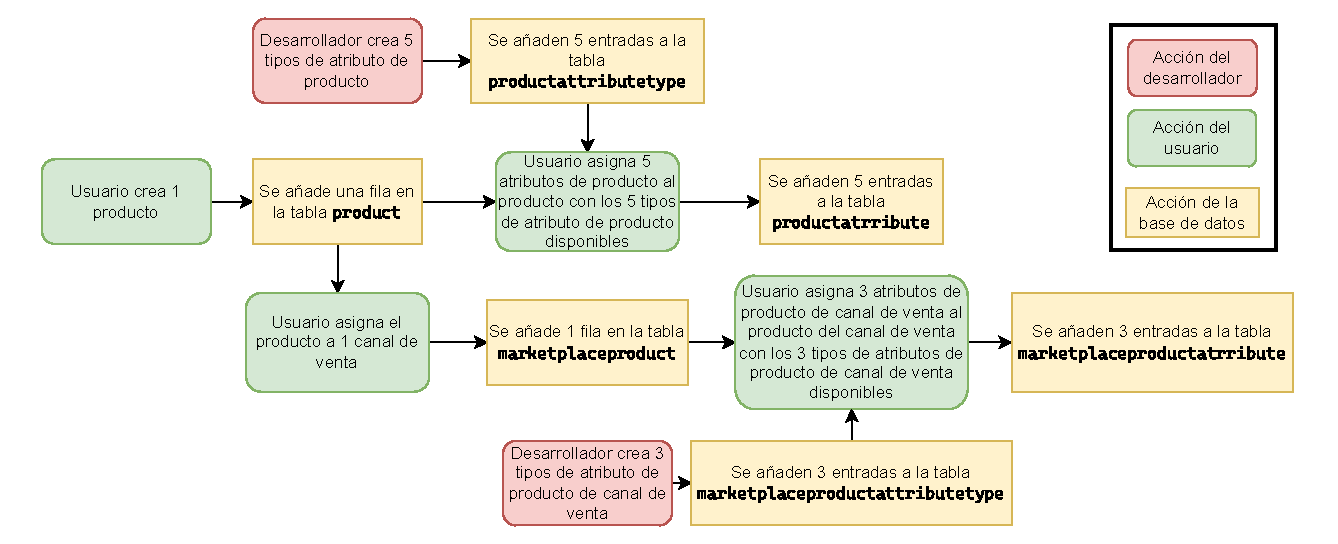
\includegraphics[width=0.8\textwidth]{figures/design_develop/products_db_diagram.pdf}
    \caption{Esquema de flujo de creación de un producto y su vinculación con un canal de venta.}
    \label{fig:products_db_diagram}
\end{figure}

Por último, en las tablas de atributos, tanto de productos como de productos del canal de venta, se ha decidido hacer una columna para cada tipo de valor, es decir, una columna por si el valor es un número, una cadena de caracteres, una fecha, etc. Dichas columnas van acompañadas otra columna, llamada \texttt{data\_type} que indica el tipo de valor, de manera que se puede saber que columna contiene el valor del atributo. El tipo de atributo también tiene una columna \texttt{data\_type}, de manera que deben ser ambos coincidentes. Así pues, a modo de ejemplo, si el tipo de atributo es "Talla", el \texttt{data\_type} será "Número" y su entrada tendrá todas las columnas vacías exceptuando la columna \texttt{data\_int}.

\begin{figure}
    \centering
    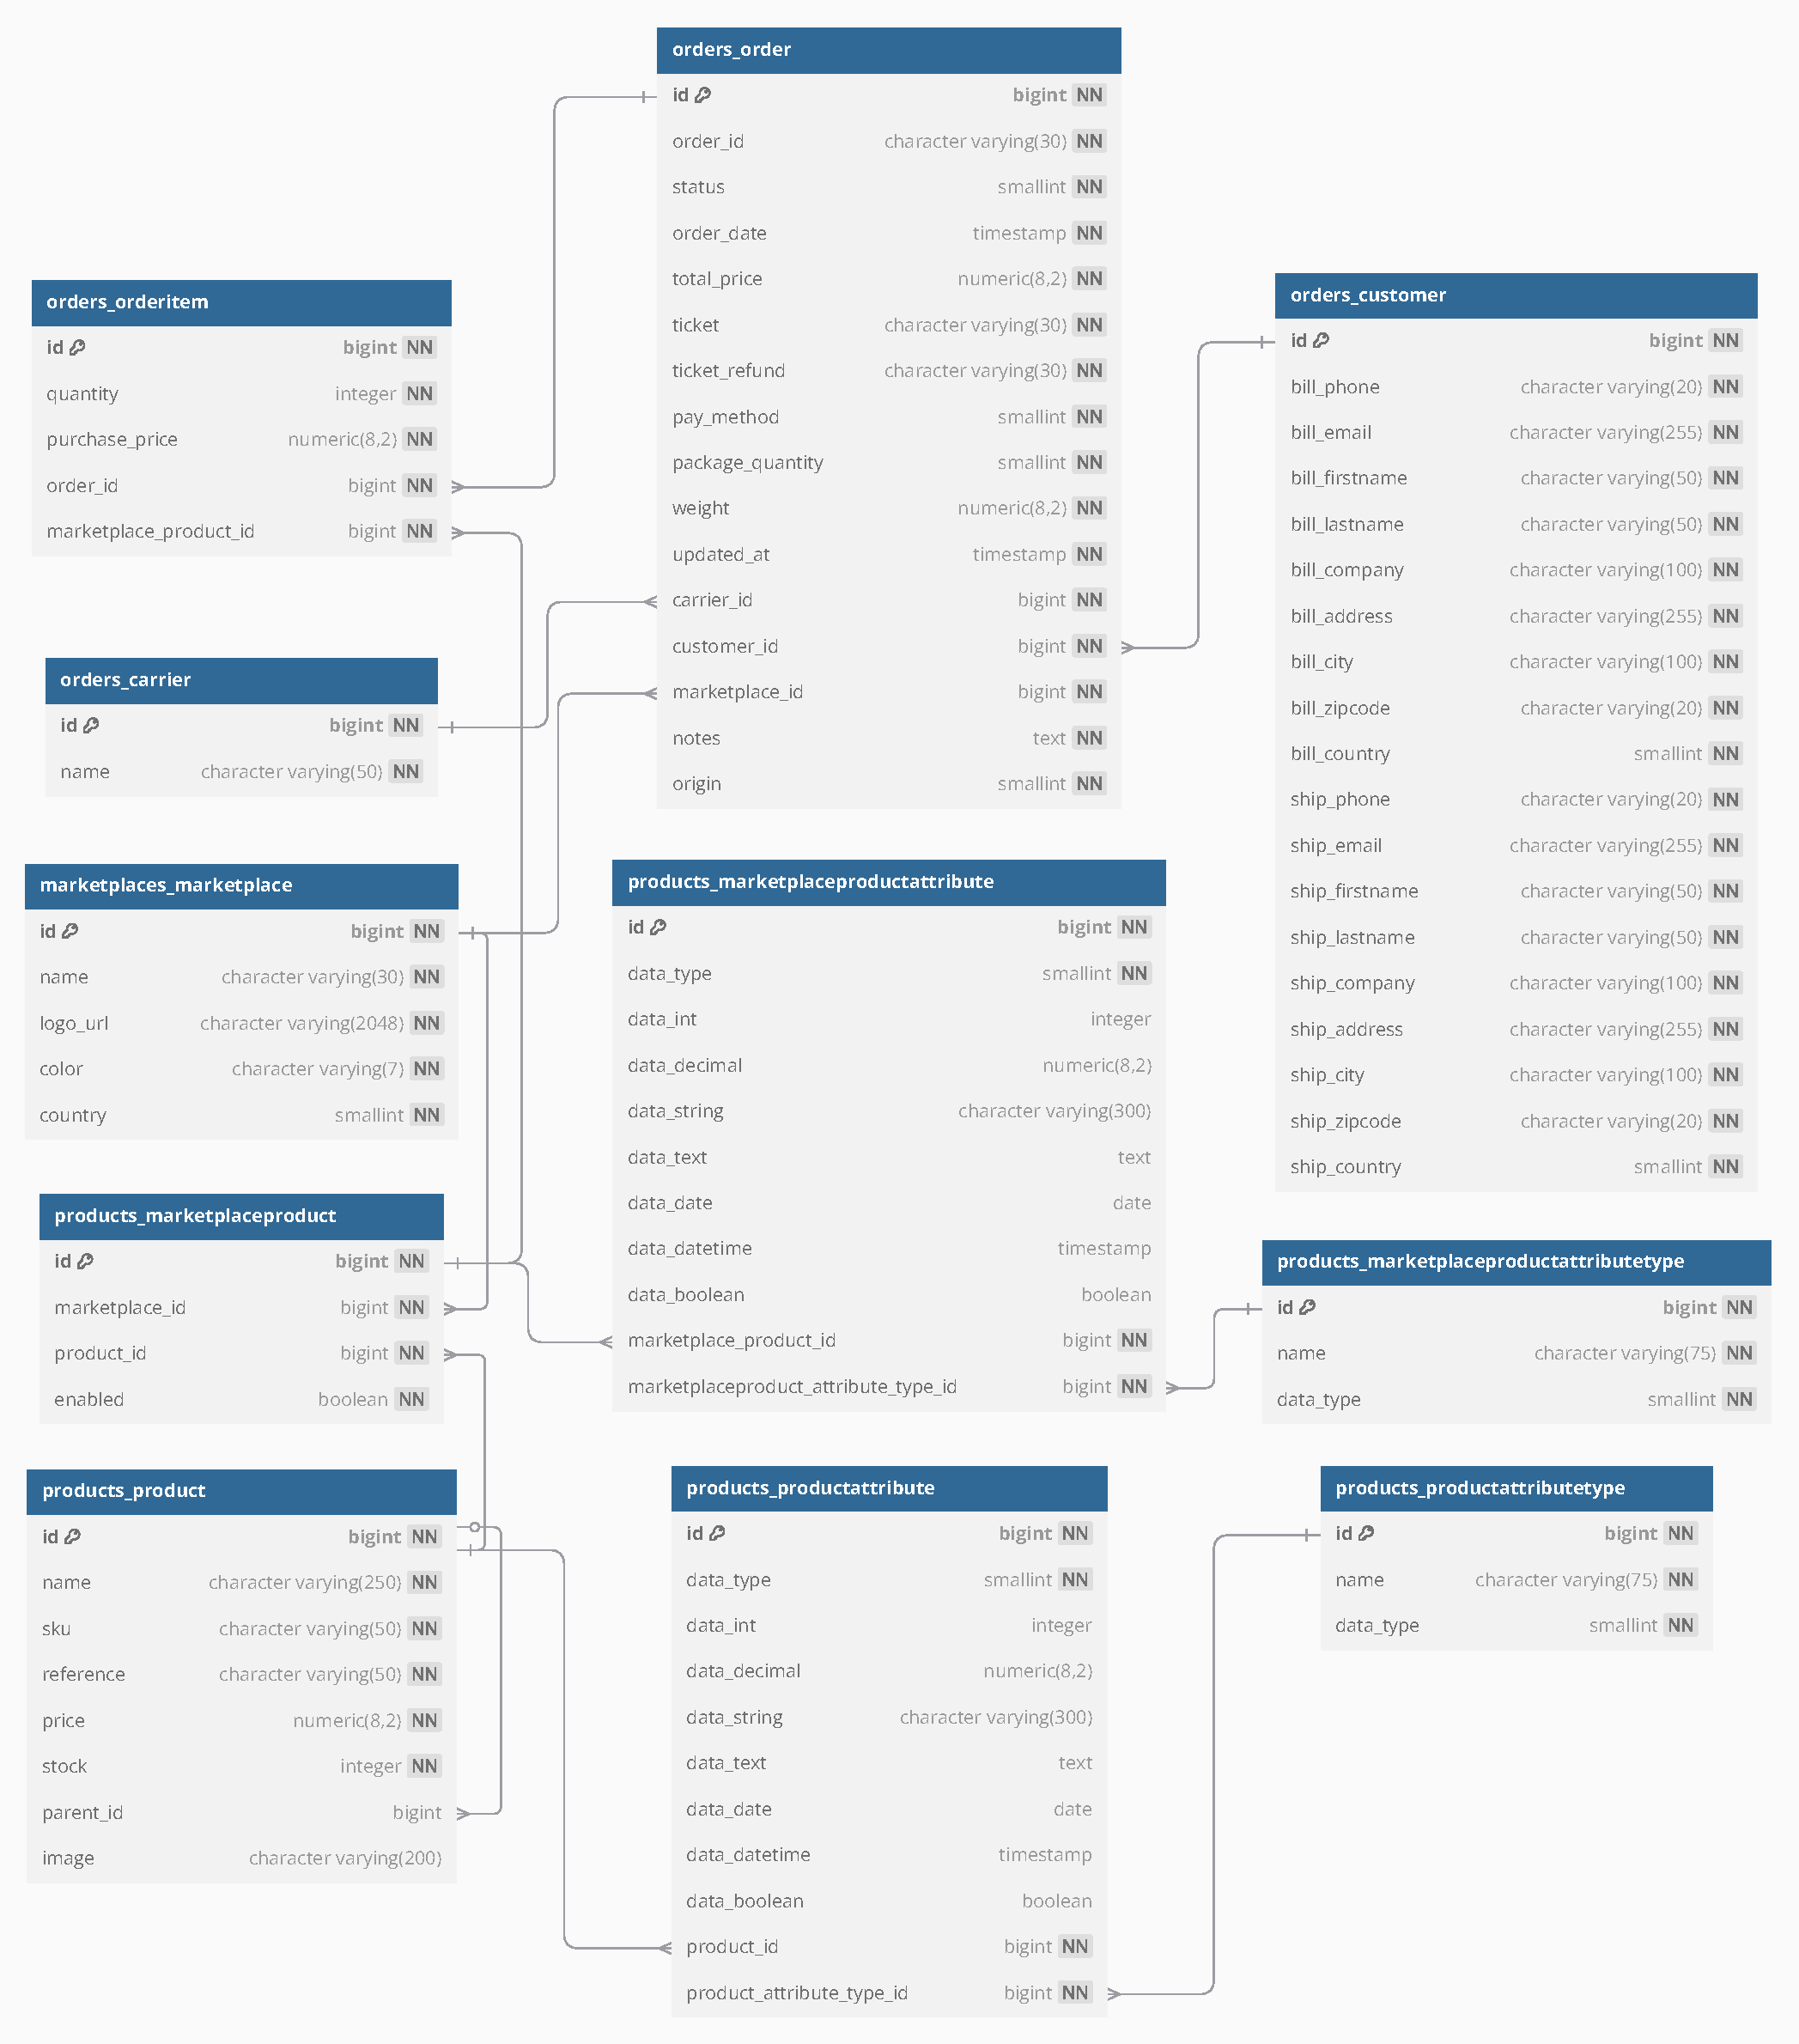
\includegraphics[width=0.98\textwidth]{figures/design_develop/database_diagram.pdf}
    \caption{Diagrama de la base de datos}
    \label{fig:diagrama_base_datos}
\end{figure}

\section{Desarrollo del \textit{backend}}


\section{Desarrollo del \textit{frontend}}
\chapter{Resumen del Presupuesto del Proyecto}
\label{ch:presupuesto}

En esta sección se presenta un resumen del presupuesto del proyecto, que incluye los costes de personal estimados para el desarrollo de esta primera versión del proyecto. El coste relacionado con el software y las herramientas utilizadas ha sido considerado nulo, ya que se ha hecho uso de software libre y gratuito.

Por otro lado, no se ha considerado ningún coste relacionado con la infraestructura, pues el despliegue de la aplicación se encuentra fuera del alcance del proyecto. Para hacer una estimación de sus costes se debería tener la aplicación desarrollada al completo y se debería hacer un estudio muy detallado de la arquitectura y de la infraestructura necesaria para su despliegue.

Con todo esto presente, el resumen del presupuesto del proyecto es el descrito en la tabla \ref{tab:presupuesto}.

\renewcommand{\arraystretch}{1.5}

\begin{table}[H]
    \centering
    \begin{tabular}{lc}
        \hline
        \textbf{Tipo}     & \textbf{Precio final}            \\
        \hline \hline
        \multicolumn{2}{c}{\textbf{DESARROLLO}}              \\
        \hline
        Base de datos     & 525 €                            \\
        \textit{Backend}  & 1050 €                           \\
        \textit{Frontend} & 2850 €                           \\
        \hline
        \multicolumn{2}{c}{\textbf{SOFTWARE Y HERRAMIENTAS}} \\
        \hline
        Software          & 0 €                              \\
        Herramientas      & 0 €                              \\
        \hline
        \textbf{TOTAL}    & \textbf{4425 €}                  \\
        \hline
    \end{tabular}
    \caption{Costes totales del proyecto.}
    \label{tab:presupuesto}
\end{table}

Alternativamente, se puede ver el presupuesto del proyecto en formato gráfico en la figura \ref{fig:presupuesto}.

\begin{figure}[H]
    \centering
    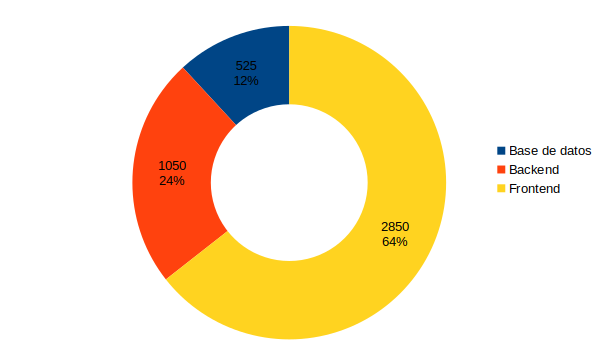
\includegraphics[width=0.8\textwidth]{figures/presupuesto/plot.png}
    \caption{Presupuesto del proyecto.}
    \label{fig:presupuesto}
\end{figure}

Por último, para una mejor comprensión de los costes del proyecto, se ha realizado un desglose detallado en el correspondiente documento de "Presupuesto", disponible en el mismo repositorio del proyecto. En este documento se pueden encontrar todos los las tareas asociadas a cada uno de los costes, así como una estimación más detallada de los tiempos invertidos en cada una de ellas. Por último, también se ha incluido en dicho documento un listado con todos los recursos de software y herramientas utilizadas.
\chapter{Análisis y valoración de las Implicaciones Ambientales y Sociales}
\label{ch:ambiental_social}

En esta sección se analizan y valoran los posibles impactos ambientales y sociales derivados del proyecto. Se busca analizar los efectos en las cuatro fases del ciclo de vida del proyecto: desarrollo, ejecución, vida útil y fin de vida. Para cada fase, se identifican los impactos ambientales y sociales, se proponen medidas de mitigación y se valoran.

Este análisis busca no solo detectar riesgos potenciales, sino también destacar oportunidades para contribuir positivamente a un desarrollo más sostenible y responsable en el ámbito del desarrollo de software y, en cierta medida, de la gestión de \textit{marketplaces}.


\section{Implicaciones Ambientales}
\label{as:sec:ambiental}

La evaluación de las implicaciones ambientales derivadas del proyecto debe identificar y valorar los impactos, tanto positivos como negativos, en el medio ambiente a lo largo de su ciclo de vida. Adicionalmente, debe estudiar las medidas a considerar para prevenir dichos impactos negativos y potenciar los positivos.

En las siguientes secciones se analizan y valoran las implicaciones ambientales en cada una de las fases del ciclo de vida del proyecto, así como las medidas de mitigación propuestas.

\subsection{Fase de desarrollo}

Al tratarse de un proyecto de desarrollo de software, el impacto ambiental más relevante en esta fase es el consumo de energía eléctrica por el uso de equipos informáticos. Sin embargo, de manera indirecta, este consumo lleva asociado un impacto ambiental derivado de la generación de energía eléctrica: la generación de gases de efecto invernadero.

Para mitigar el posible impacto derivado del consumo de energía eléctrica, se ha tratado de hacer un uso eficiente de los equipos informáticos, evitando el uso de equipos innecesarios, como pueden ser servidores de desarrollo, y apagando los equipos cuando no se están utilizando. Por otro lado, cabe remarcar que toda la documentación del proyecto se ha realizado de manera digital, evitando el uso de papel y reduciendo así el impacto ambiental asociado a la impresión de documentos.

Con todo esto presente, se puede estimar que los impactos ambientales en esta fase son controlables y relativamente bajos, únicamente asociados al consumo energético individual de mi persona.

\subsection{Fase de ejecución}

En esta segunda fase se contempla el impacto ambiental derivado a la implementación del software desarrollado a los medios de comunicación y almacenamiento necesarios para su funcionamiento. En este caso, al tratarse de una aplicación web, el impacto ambiental más relevante es el consumo energético asociado a los servidores que alojan la aplicación y a la infraestructura de red necesaria para su funcionamiento.

Para tratar de reducir al máximo este impacto, se contempla hacer una optimización del código, evitando el uso de recursos innecesarios y haciendo un uso eficiente de las consultas a bases de datos. Como mayor sea la eficiencia del código, menor será el consumo energético asociado a su ejecución.

Consecuentemente, se puede estimar que el impacto ambiental en esta fase es moderado, ya que depende de la eficiencia del código y de la infraestructura utilizada para alojar la aplicación.

\subsection{Vida útil}

En esta tercera fase, el paradigma ya cambia considerablemente. Al tratarse de una aplicación web, todo el software desarrollado debe ser ejecutado en un servidor, el cual debe estar encendido y funcionando las 24 horas del día. Esto implica un consumo energético constante, que puede ser significativo dependiendo de la infraestructura utilizada.

Para tratar de mitigar estos impactos, se contempla realizar una buena elección de proveedores de servicios en la nube, los cuales demuestren un compromiso con la sostenibilidad, haciendo uso de energías renovables y poseyendo certificaciones de eficiencia energética.

De esta manera, en la fase de vida útil hay cierto traslado de responsabilidad hacia el proveedor de servicios en la nube, ya que la sostenibilidad del proyecto dependerá en gran medida de las prácticas ambientales de dicho proveedor. Sin embargo, se debe tratar de hacer la elección más responsable posible, pues es la fase con un mayor impacto.

\subsection{Fin de vida}

En la fase final del ciclo de vida del proyecto, se debe considerar el impacto ambiental derivado de la eliminación del software y de la infraestructura utilizada para su funcionamiento. En este caso, el impacto más relevante es el asociado a los residuos electrónicos generados por los servidores y otros equipos utilizados para alojar la aplicación.

La mitigación de este impacto va también bastante ligada a la elección de proveedores de servicios en la nube, ya que muchos de ellos ofrecen servicios de reciclaje y reutilización de equipos electrónicos. Además, se debe considerar la posibilidad de migrar el software a nuevas infraestructuras más sostenibles, evitando así la generación de residuos innecesarios.

Así pues, el impacto ambiental en esta fase puede ser significativo, pero también es controlable y mitigable mediante la elección de proveedores responsables y prácticas de reciclaje adecuadas. Mantenerse actualizado con nuevos proveedores y tecnologías sostenibles puede ayudar a reducir el impacto ambiental en esta fase.

\section{Implicaciones Sociales}
\label{as:sec:sociales}

La evaluación de las implicaciones sociales del proyecto debe identificar y valorar los impactos, tanto positivos como negativos, en la sociedad a lo largo de su ciclo de vida. Debe valorar todos aquellos aspectos éticos y de género que puedan surgir durante el desarrollo del proyecto, así como los posibles impactos en la comunidad y en los usuarios finales de la aplicación. Por último, debe estudiar las medidas a considerar para prevenir dichos impactos negativos y potenciar los positivos.

En las siguientes secciones se analizan y valoran las implicaciones sociales en cada una de las fases del ciclo de vida del proyecto, así como las medidas de mitigación propuestas. Al no haber gran diferencia entre la fase de ejecución y la fase de vida útil, se tratarán conjuntamente.

\subsection{Fase de desarrollo}

En la fase de desarrollo, el impacto social es más bien limitado, ya que el proyecto se desarrolla de manera individual. Sin embargo, es importante considerar aspectos éticos y de género en el desarrollo del software, como la accesibilidad y la inclusión de diferentes grupos sociales.

Para mitigar posibles impactos negativos, se ha tratado de seguir buenas prácticas de desarrollo, como el uso de herramientas de control de versiones y la documentación del código. Además, se ha procurado que el software sea accesible y usable para diferentes grupos sociales, teniendo en cuenta aspectos como la diversidad funcional y la inclusión de personas con discapacidad.

\subsection{Fase de ejecución y Vida útil}

En esta fase, el impacto social puede ser más relevante. Se identifican diversos impactos sociales, principalmente positivos. La plataforma facilita la expansión de negocios al reducir la complejidad operativa de gestionar múltiples canales de venta, lo que favorece la inclusión de pequeños comerciantes sin conocimientos técnicos avanzados. Además, optimiza la gestión del trabajo, permitiendo que los empleados se centren en tareas de mayor valor estratégico. A nivel social, también contribuye a la mejora de la calidad de vida de los usuarios al simplificar procesos rutinarios, y refuerza la accesibilidad mediante una interfaz centrada en la usabilidad para todos los perfiles.

Para maximizar estos beneficios y mitigar los posibles riesgos, se pretende aplicar un conjunto de medidas para cada uno de los impactos. En materia de seguridad y ética, se pretende desarrollar un sistema de autenticación robusto que protege los datos sensibles de clientes y pedidos, reduciendo el riesgo de accesos no autorizados. Asimismo, se planea poner especial atención en evitar sesgos en la representación de datos y en asegurar la escalabilidad del sistema para adaptarse a nuevas funcionalidades sin excluir a nuevos usuarios.

En definitiva, el impacto de la plataforma durante su ejecución y operación puede considerarse positivo, tanto desde una perspectiva social como funcional. Su diseño centrado en la accesibilidad, la automatización y la seguridad promueve un entorno más equitativo y eficiente.

\subsection{Fin de vida}

En la fase final del ciclo de vida del proyecto, el principal impacto identificado está relacionado con el cese de operaciones de la aplicación y sus consecuencias para los usuarios. La interrupción del servicio podría generar dificultades para los comercios que dependan de la plataforma para gestionar sus operaciones diarias, además del riesgo potencial de pérdida de datos relevantes como historiales de productos, pedidos o información de clientes.

Para mitigar este impacto, se contempla la implementación de procedimientos claros de finalización del servicio. Estos incluirán la notificación con antelación suficiente a todos los usuarios para que puedan realizar una migración. En caso de que los usuarios no requieran esta migración, se garantizará la eliminación definitiva de la información, cumpliendo estrictamente con las normativas de protección de datos y privacidad vigentes.

En conjunto, aunque el fin de vida de la plataforma podría tener un impacto sensible en la operativa de los usuarios, una planificación anticipada y responsable permitiría gestionarlo de forma ética y controlada.

\chapter{Conclusiones}
\label{chap:conclusiones}

\newpage
\printbibliography

\end{document}